\pagebreak
\subsection{Moment of Inertia} %\label{put a label here and uncomment}
\textbf{Name: Group 510}\\
\textbf{Date: 30/09 - 2015}

\subsubsection{Purpose}
The purpose of this test is to find the moment of inertia $I$, by measuring the motor velocity as a function of time.

\subsubsection{Setup}
\begin{figure}[H]
  \centering
	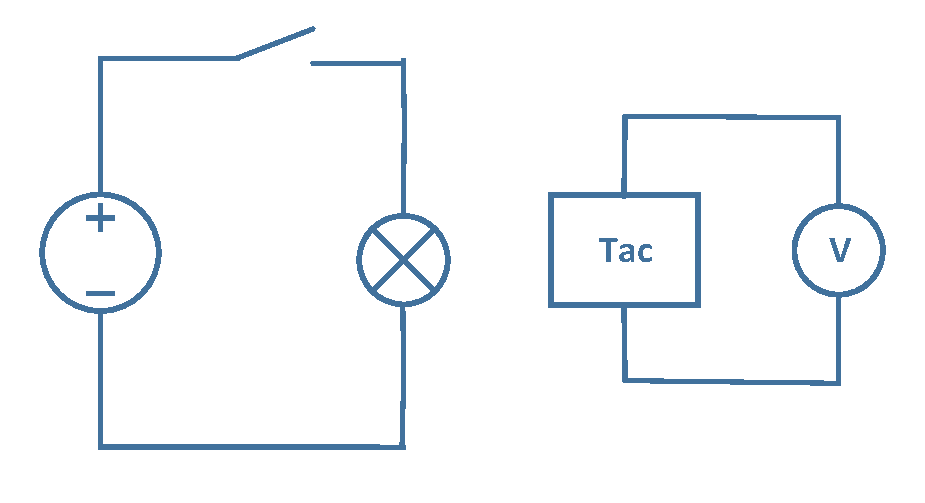
\includegraphics[scale=0.5]{figures/MotorTest7.pdf}
	\caption{Setup diagram}
\end{figure}

\subsubsection{List of Equipment}

\begin{table}[H]
\begin{tabular}{|l|l|p{4cm}|}
\hline%------------------------------------------------------------------------------------
  \textbf{Instrument}                        &  \textbf{AAU-no.}  &  \textbf{Type}       \\
\hline%------------------------------------------------------------------------------------
  Oscilloscope                               &  64672             &  Agilent DSO6034A    \\
\hline%------------------------------------------------------------------------------------
  Power Supply ($0 - 32$ V) ($0 - 10$ A)     &  77076             &  Ea - ps 7032 - 100  \\
\hline%------------------------------------------------------------------------------------
  Optical tachometer                         &  77087             &  Compact             \\
\hline%------------------------------------------------------------------------------------
\end{tabular}
\end{table}

\subsubsection{Procedure}

\begin{enumerate}
  \item Turn on the oscilloscope.
  \item On the oscilloscope press the "mode"-key choose the "normal"-option, set the trigger to "falling edge".
  \item To prevent false triggering on the oscilloscope set the trigger value to %\fxnote{input value from extracted data} mV with the turn-key.
  \item Turn on the power supply at 7 volt.
  \item Press "single"-key on oscilloscope and cut the power of the motor.
  \item Insert a USB-pin in the oscilloscope and press the save key to extract the data.
\end{enumerate}

\subsubsection{Results}

\begin{figure}[H]
  \setcounter{subfigure}{0}
  \centering
  \begin{subfigure}{0.45\textwidth}
    \centering
    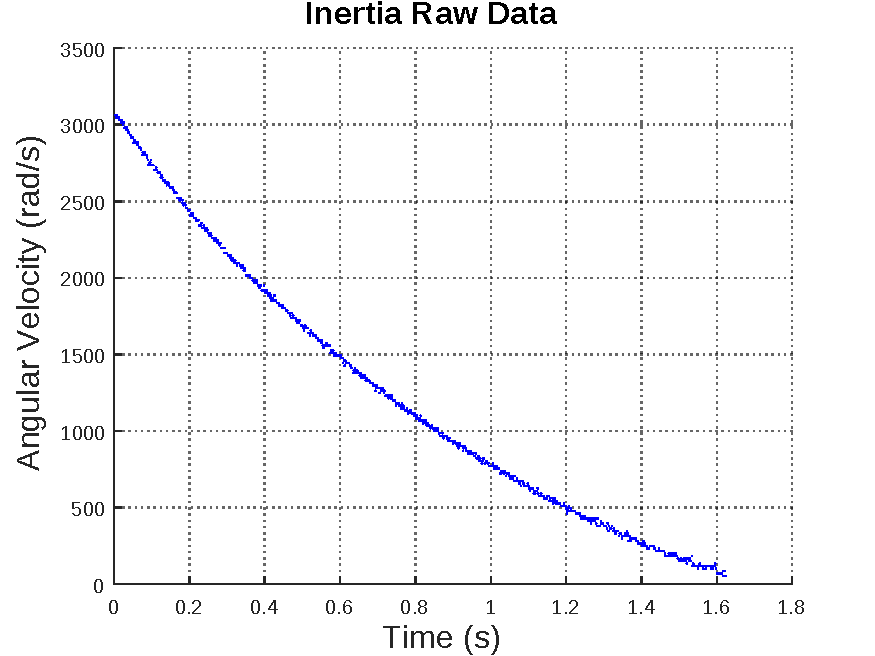
\includegraphics[width=1.1\linewidth]{figures/inertiaRawData.pdf}
    \caption{Plot of test results}
    \label{momentOfInertia}
  \end{subfigure}
  \begin{subfigure}{0.45\textwidth}
    \centering
    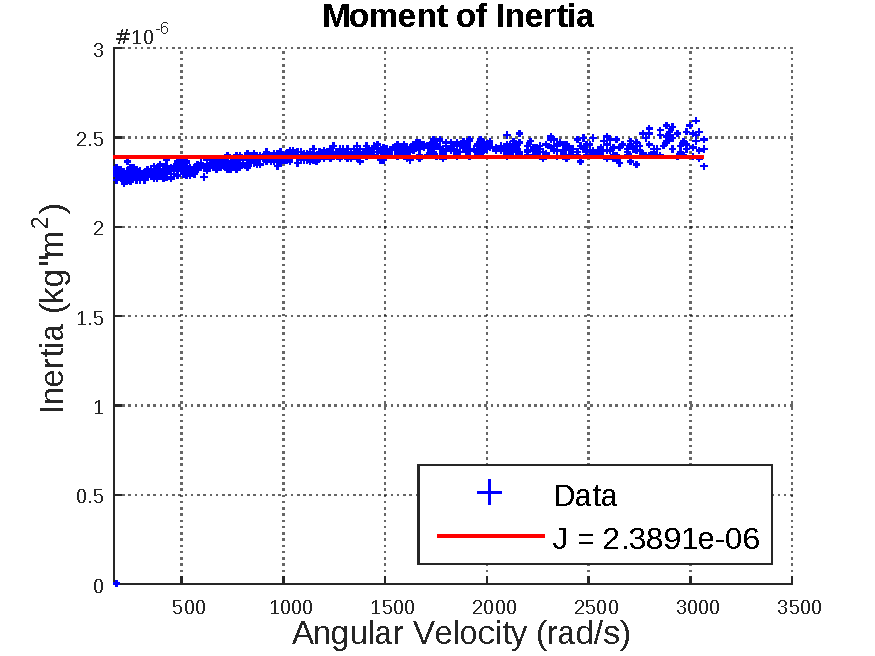
\includegraphics[width=1.1\linewidth]{figures/momentOfInertia.pdf}
    \caption{Plot of the moment of inertia}
  	\label{inertiaRawData}
  \end{subfigure}
  \caption{hey}
  \label{yo}
\end{figure}
\todo{make text on figure larger}

The following equation which arises from the mechanical description of the motor when \si{i_a = 0} is given in the Modeling and Control course on the 5th semester on Electronic and IT on Aalborg University.
\begin{align}
  \eq{\omega(s)}{- \frac{\tau_c}{B}+(\omega_0 + \frac{\tau_c}{B}) e^{-t\frac{B}{J}}} \unit{rad\cdot s^{-1}}\nonumber\\
  && &\Updownarrow&&\\
  \eq{J}{ \frac{B\cdot t}{ln(  \frac{B\cdot \omega_0 + \tau_c}{B \cdot \omega + \tau_c})} } \unit{N\cdot m}\nonumber
\end{align}




